\chapter{PLANTEAMIENTO DEL PROBLEMA}
\section{Descripción de la Realidad Problemática}

Las discapacidades del habla abarcan una amplia gama de condiciones que afectan la capacidad de una persona para comunicarse verbalmente de manera clara y fluida. Según la American Speech-Language-Hearing Association (ASHA), las discapacidades del habla pueden originarse por una variedad de razones, que van desde dificultades físicas en los órganos responsables de la producción del habla, hasta trastornos neurológicos que impactan la habilidad de hablar de manera clara y fluida.

Para las personas con discapacidades del habla, el lenguaje de señas se convierte en una herramienta invaluable que les permite expresar sus pensamientos, emociones y necesidades de manera efectiva. El lenguaje de señas es un sistema de comunicación visual y gestual utilizado por personas sordas o con discapacidades auditivas para comunicarse entre sí y con personas que pueden escuchar.

La Organización Mundial de la Salud afirmó que aproximadamente 70 millones de personas en el mundo son sordomudas. Un total de 360 millones de personas son sordas, y 32 millones de ellas son niños. Sin embargo, en Perú, de acuerdo con los resultados del Censo de Población y Vivienda 2017, como se puede observar en la Figura \ref{1:fig 1}, hay un elevado porcentaje de personas que tienen dificultades para oír y para hablar o comunicarse.

El INEI también afirma que las personas presentan estas capacidades utilizan como apoyo para comunicarse su voz (19,8\% ), gesto y manos (11,9\% ) y lenguaje de señas (2,9\% ). Y debido a estas dificultades, estas personas se ven afectadas en el ámbito social y también laboral, por no poder expresarse debido a sus discapacidades. Según la Organización Mundial de Salud, las personas con estas discapacidades tienen más probabilidades de experimentar pobreza y exclusión social, y tienen menos probabilidades de tener un empleo remunerado que las personas sin discapacidades. En base a encuestas realizadas por la organización Incluyeme, alrededor del 72\% de personas con discapacidad se encuentra desempleado, como se puede observar en la Figura \ref{1:fig 2}.

El objetivo principal de esta investigación es lograr un aumento significativo en la comunicación entre personas con discapacidades del habla y aquellas que no las tienen, a través de la implementación de un modelo de traducción de lenguaje de señas utilizando Deep Learning. Este modelo busca facilitar una interacción más fluida y efectiva, permitiendo a las personas con discapacidades del habla expresar sus pensamientos, emociones y necesidades de manera más accesible y comprensible para quienes no conocen el lenguaje de señas.

\begin{figure}[h]
	\begin{center}
		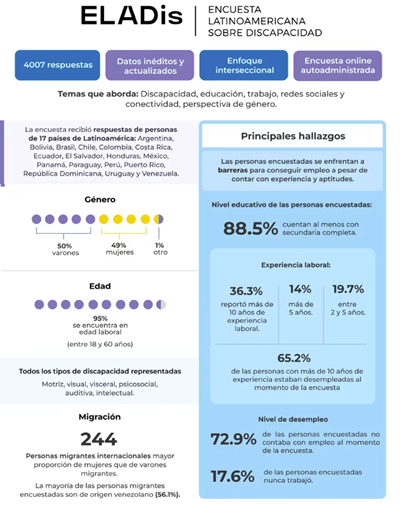
\includegraphics[width=0.5\textwidth]{1/figures/Encuesta_personas_discapacidad.png}
		\caption{Encuesta de personas con discapacidad . Fuente: \cite{encuesta_personas_discapacidad}}
		\label{1:fig 2}
	\end{center}
\end{figure}

\begin{figure}[h]
	\begin{center}
		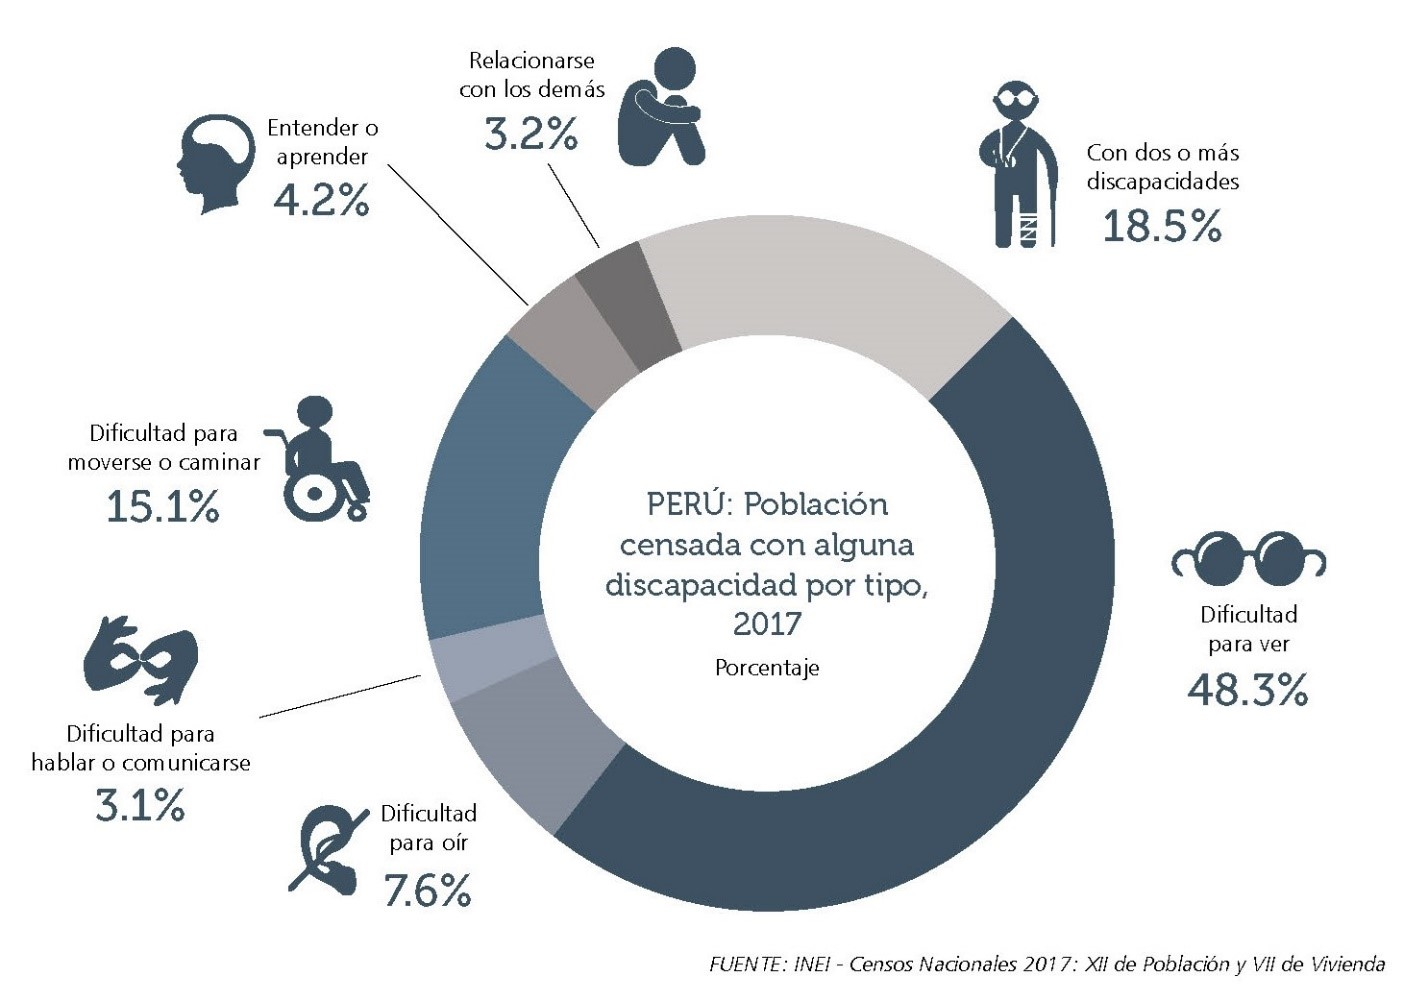
\includegraphics[width=0.5\textwidth]{1/figures/personas_discapacidad.jpg}
		\caption{\% de personas con discapacidad. Fuente: \cite{porcentaje de_personas_discapacidad}}
		\label{1:fig 1}
	\end{center}
\end{figure}




\section{Formulación del Problema}


\subsection{Problema General}
\newcommand{\ProblemaGeneral}{
	El problema general de esta investigación es la Dificultad de comunicación para personas con indiscapacidades del habla al interactuar con personas que no conocen el lenguaje de señas.
}
\ProblemaGeneral
\subsection{Problemas Espec\'{i}ficos}
\newcommand{\Pbone}{
¿Cómo pueden los modelos de Deep Learning leer e interpretar el lenguaje de señas?
}
\newcommand{\Pbtwo}{
¿Cómo los modelos de Deep Learning pueden predecir lenguaje de señas para una conversación fluida entre una persona con discacidad y otra sin ninguna?
}
\newcommand{\Pbthree}{
¿De que manera los modelos Deep Learning pueden  diferenciar entre los distintos tipos de lenguajes de señas?
}

\begin{itemize}
	\item \Pbone
	\item \Pbtwo
	\item \Pbthree
\end{itemize}

\section{Objetivos de la Investigación}
\subsection{Objetivo General}
\newcommand{\ObjetivoGeneral}{
Mediante el modelo de Deep Learning se utilizará una herramienta de traducción entre personas con discapacidades del habla que utilizan lenguaje de señas con personas que no conocen este lenguaje. 
}
\ObjetivoGeneral
\subsection{Objetivos Espec\'{i}ficos}
\newcommand{\Objone}{
Traducir lenguajes de señas utilizando técnicas de visión de computadora y el uso de Redes Neuronales.
}
\newcommand{\Objtwo}{
El modelo puede ser entrenado utilizando conjuntos extensos de datos para mejorar su exactitud y capacidad de interpretación de gestos. Esto facilita una comunicación más natural y sin interrupciones entre individuos con y sin discapacidad auditiva.
}
\newcommand{\Objthree}{
Los modelos de Deep Learning pueden entrenarse con conjuntos de datos etiquetados que contienen ejemplos de diferentes lenguajes de señas. Esto les permite aprender a asociar patrones visuales específicos con cada lenguaje de señas.
}

\begin{itemize}
	\item {\Objone}
	\item {\Objtwo}
	\item {\Objthree}
\end{itemize}

\section{Justificación de la Investigación}

\subsection{Teórica}
Esta investigación se realiza 

\subsection{Práctica}
Al culminar la investigación 

\subsection{Metodológica}. 

\section{Delimitación del Estudio}

\subsection{Espacial}
Para la presente investigación 

\subsection{Temporal}
Los datos que serán necesari. 

\subsection{Conceptual}
Esta investigación se 

\section{Hipótesis}

\subsection{Hipótesis General}
\newcommand{\HipotesisGeneral}{
El uso de técnicas de.
}
\HipotesisGeneral
\subsection{Hipótesis Específicas}
\newcommand{\Hone}{
	x
}
\newcommand{\Htwo}{
	y
}
\newcommand{\Hthree}{
	z	
}
\newcommand{\Hfour}{
	cv
}
\newcommand{\Hfive}{
	xws
}
\begin{itemize}
	\item \Hone
	\item \Htwo
	\item \Hthree
	\item \Hfour
	\item \Hfive
\end{itemize}

\subsection{Matriz de Consistencia}
A continuación se presenta la matriz de consistencia elaborada para la presente investigación (véase Anexo \ref{1:table}).

